%%%%%%%%%%%%%%%%%%%%%%%%%%%%%%%%%%%%%%%%%%%%%%%%%%%%%%%%%%%

\chapter{Modello del sistema - gruppo 5}
\label{ref:modSistemaGruppo5}

%%% Il gruppo 5 scriverà il suo modello del sistema. Esso dovrà includere: attori, casi d'uso (descrizione e tabella), scenari, diagrammi dei casi d'uso, diagrammi di sequenza, diagramma delle attività, screen mockups della funzionalità %%%

\section{Attori}
\paragraph{Studente:} è colui che una volta effettuato il login, avrà accesso ai contatti dell'unimol passando per la sezione rubrica.

\paragraph{Esse3:} il consorzio universitario Cineca, nell’ambito dell’applicazione da sviluppare svolgerà il compito cruciale di fornire (e quindi comunicare con l’app stessa) le informazioni riguardanti i contatti dei professori, nonché la segreteria.

\section{Casi d'uso}

\paragraph{Precondizione\\} 
Lo \textit{Studente} deve aver effettuato il login per accedere ai servizi dell'app Studenti Unimol.

\clearpage

\paragraph{Ricerca non filtrata \\} 
Il caso d'uso mostra, nella tabella sottostante, il comportamento
che il sistema assume quando lo \textit{Studente} accede alla sezione rubrica e non effettua nessun tipo di ricerca.

\begin{table}[!h]
	%\normalsize % Dimensione testo normale
	\small % Dimensione testo piccola
	%\footnotesize % Dimensione testo piccolissima
	%\scriptsize % Dimensione del testo ulteriormente più piccola
	 % Didascalia tabella
	\label{tab:template-tab-casiduso-tre-attori} % Etichetta per riferimenti incrociati
	\begin{tabular}{| p{\useCaseLeft} | p{\useCaseNum} | p{\useCaseThreeCol} | p{\useCaseThreeCol} | p{\useCaseThreeCol} |}
		\hline
		\textbf{Nome caso d'uso} & \multicolumn{4}{p{\useCaseMulticol} |}{\textbf{Ricerca non filtrata}} \\
		\hline
		\textbf{Attori partecipanti} & \multicolumn{4}{p{\useCaseMulticol} |}{Inizializzato da \textbf{Studente}. Partecipa \textbf{Esse3}.} \\
		\hline
		\textbf{Condizioni d'ingresso} & \multicolumn{4}{p{\useCaseMulticol} |}{Lo \textit{Studente} accede alla sezione della rubrica.} \\
		\hline
		\textbf{Flusso degli eventi} & \textbf{\#} & \textbf{Studente} & \textbf{Sistema} & \textbf{Esse3} \\
		\hline
		\textbf{} & \textbf{1} & \textbf{} & Richiede la lista completa dei contatti ad \textit{Esse3}. & \textbf{} \\
		\hline
		\textbf{} & \textbf{2} & \textbf{} & \textbf{} & Elabora la richiesta e invia i dati relativi alla rubrica. \\
		\hline
		\textbf{} & \textbf{3} & \textbf{} & Mostra allo \textit{Studente} l'elenco dei contatti in rubrica. & \textbf{} \\
		\hline
		\textbf{Eccezioni} & \multicolumn{4}{p{\useCaseMulticol} |}{3.1 \textit{Esse3} non risponde.\newline 3.2 Connessione assente: il sistema restituisce l'ultima copia salvata in locale. \newline 3.3 Connessione assente e copia non presente.} \\
		\hline
		\textbf{Condizioni d'uscita} & \multicolumn{4}{p{\useCaseMulticol} |}{Lo \textit{Studente} visualizza tutti i contatti della rubrica.} \\
		\hline
	\end{tabular}
\caption{Rubrica - Ricerca non filtrata}
\end{table}

\newpage

\paragraph{Ricerca filtrata \\} 
Il caso d'uso è il più frequente e mostra nella tabella sottostante il comportamento che il sistema assume quando lo \textit{Studente}
cerca informazioni inerenti un docente o il personale di segreteria di una sede didattica specifica.

\begin{table}[!h]
	%\normalsize % Dimensione testo normale
	\small % Dimensione testo piccola
	%\footnotesize % Dimensione testo piccolissima
	%\scriptsize % Dimensione del testo ulteriormente più piccola
	 % Didascalia tabella
	\label{tab:template-tab-casiduso-tre-attori} % Etichetta per riferimenti incrociati
	\begin{tabular}{| p{\useCaseLeft} | p{\useCaseNum} | p{\useCaseThreeCol} | p{\useCaseThreeCol} | p{\useCaseThreeCol} |}
		\hline
		\textbf{Nome caso d'uso} & \multicolumn{4}{p{\useCaseMulticol} |}{\textbf{Ricerca filtrata}} \\
		\hline
		\textbf{Attori partecipanti} & \multicolumn{4}{p{\useCaseMulticol} |}{Inizializzato da \textbf{Studente}. Partecipa \textbf{Esse3}.} \\
		\hline
		\textbf{Condizioni d'ingresso} & \multicolumn{4}{p{\useCaseMulticol} |}{Lo \textit{Studente} accede alla sezione della rubrica.} \\
		\hline
		\textbf{Flusso degli eventi} & \textbf{\#} & \textbf{Studente} & \textbf{Sistema} & \textbf{Esse3} \\
		\hline
		\textbf{} & \textbf{1} & Inserisce i parametri di ricerca nella barra di ricerca che consente di inserire stringhe di testo. & \textbf{}  & \textbf{} \\
		\hline
		\textbf{} & \textbf{2} & \textbf{} & Richiede il contatto ad \textit{Esse3}. & \textbf{} \\
		\hline
		\textbf{} & \textbf{3} & \textbf{} & \textbf{} & Elabora la richiesta e invia i dati relativi alla rubrica. \\
		\hline
		\textbf{} & \textbf{4} & \textbf{} & Mostra allo \textit{Studente} il contatto cercato in rubrica. & \textbf{} \\
		\hline
		\textbf{Eccezioni} & \multicolumn{4}{p{\useCaseMulticol} |}{3.1 \textit{Esse3} non risponde.\newline 3.2 Connessione assente: il sistema restituisce l'ultima copia salvata in locale. \newline 3.3 Connessione assente e copia non presente. \newline 3.4 Contatto non presente.} \\
		\hline
		\textbf{Condizioni d'uscita} & \multicolumn{4}{p{\useCaseMulticol} |}{Lo \textit{Studente} visualizza il contatto cercato nella rubrica.} \\
		\hline
	\end{tabular}
\caption{Rubrica - Ricerca filtrata}
\end{table}

\newpage

\paragraph{Visualizza contatto \\} 
Lo \textit{Studente}, dopo aver effettuato una ricerca e aver trovato il contatto, seleziona il contatto e visualizza le informazioni. Non ci sono eccezioni in quanto la ricerca è andata a buon fine.

\begin{table}[!h]
	%\normalsize % Dimensione testo normale
	\small % Dimensione testo piccola
	%\footnotesize % Dimensione testo piccolissima
	%\scriptsize % Dimensione del testo ulteriormente più piccola
	 % Didascalia tabella
	\label{tab:template-tab-casiduso-due-attori} % Etichetta per riferimenti incrociati
	\begin{tabular}{| p{\useCaseLeft} | p{\useCaseNum} | p{\useCaseTwoCol} | p{\useCaseTwoCol} |}
		\hline
		\textbf{Nome caso d'uso} & \multicolumn{3}{p{\useCaseMulticol} |}{\textbf{Visulizza contatto}} \\
		\hline
		\textbf{Attori partecipanti} & \multicolumn{3}{p{\useCaseMulticol} |}{Inizializzato da \textbf{Studente}.} \\
		\hline
		\textbf{Condizioni d'ingresso} & \multicolumn{3}{p{\useCaseMulticol} |}{Lo \textit{Studente} ha effettuato una ricerca dalla rubrica.} \\
		\hline
		\textbf{Flusso degli eventi} & \textbf{\#} & \textbf{Utente} & \textbf{Sistema} \\
		\hline
		\textbf{} & \textbf{1} & Seleziona il contatto trovato. & \textbf{} \\
		\hline
		\textbf{} & \textbf{2} & \textbf{} & Mostra le informazioni del contatto selezionato:
			\begin{enumerate}
			\item Nome Cognome
			\item Dipartimento, Sede
			\item Email
			\item Numero telefonico
			\end{enumerate} \\
		\hline
		\textbf{Condizioni d'uscita} & \multicolumn{3}{p{\useCaseMulticol} |}{Lo \textit{Studente} visualizza le informazioni del contatto selezionato.} \\
		\hline
	\end{tabular}
\caption{Rubrica - Visualizza contatto}
\end{table}

\clearpage

\section{Diagramma dei casi d'uso}


\begin{figure}[!h]
	\centering
	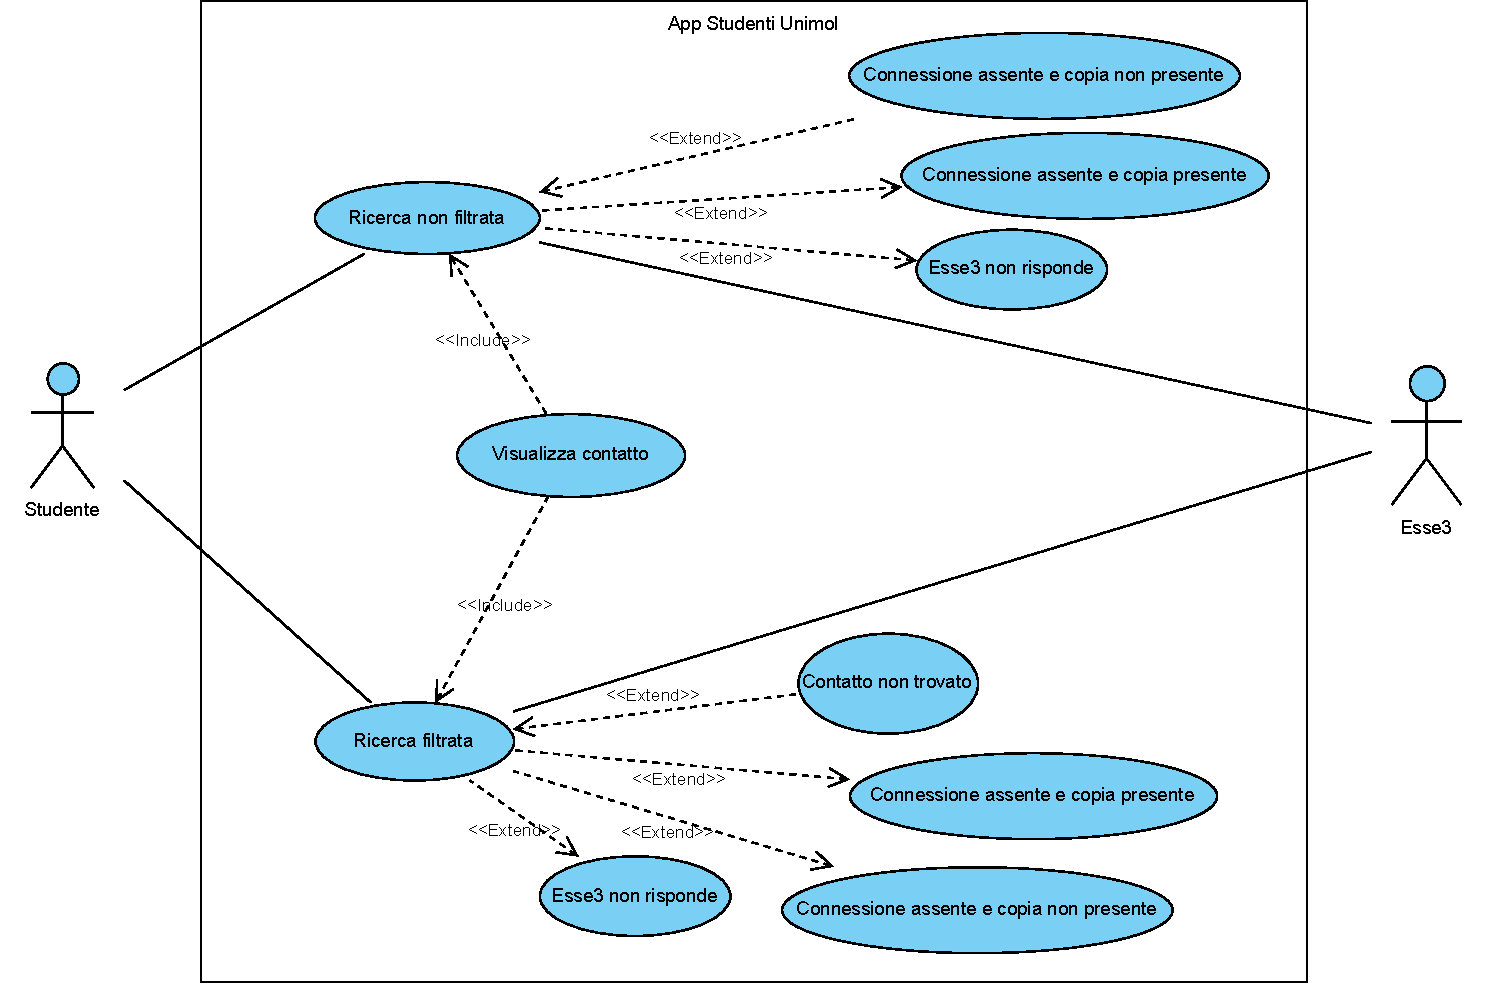
\includegraphics[height=3in]{imgs/gruppo5/Diagram1.pdf}
	\caption{Rubrica}
	\label{fig:prova}
\end{figure}


\section{Diagramma di sequenza}

\begin{figure}[!h]
	\centering
	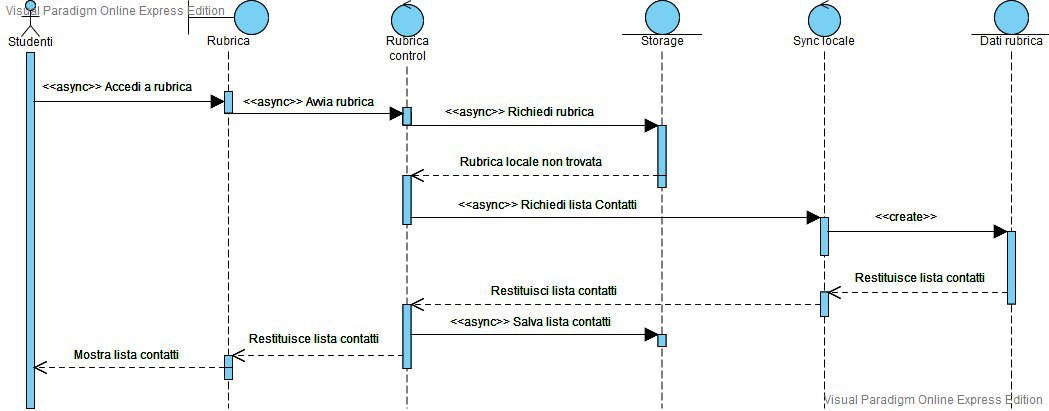
\includegraphics[height=3in,width=5in]{imgs/gruppo5/sequence1.jpg}
	\caption{Rubrica - Ricerca non filtarta}
	\label{fig:prova}
\end{figure}

\begin{figure}
	\centering
	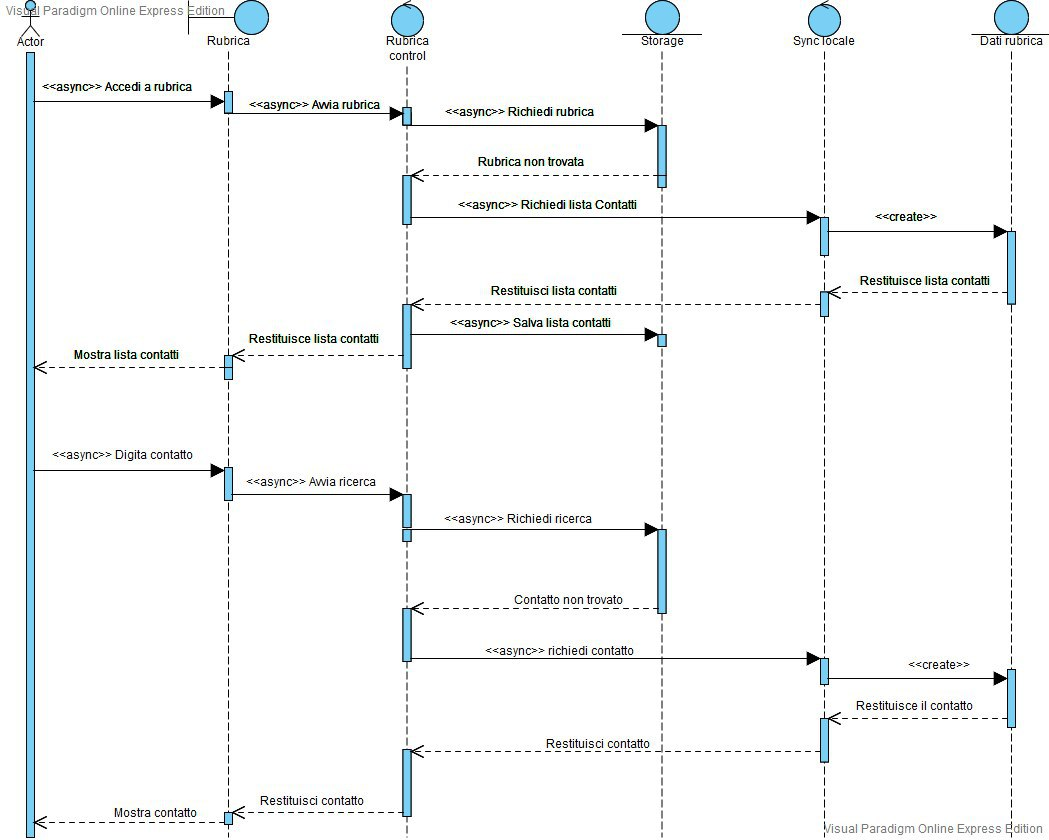
\includegraphics[height=3in,width=5in]{imgs/gruppo5/sequence3.jpg}
	\caption{Rubrica - Ricerca filtarta}
	\label{fig:prova}
\end{figure}

\begin{figure}
	\centering
	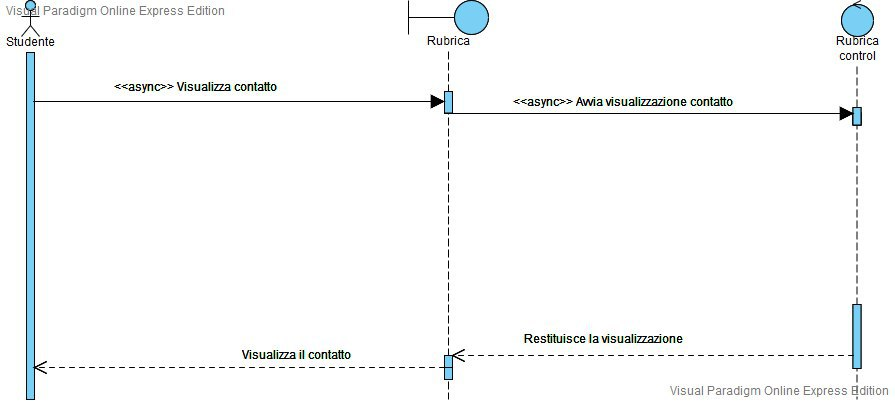
\includegraphics[height=3in,width=5in]{imgs/gruppo5/sequence2.jpg}
	\caption{Rubrica - Visualizza contatto}
	\label{fig:prova}
\end{figure}

\clearpage

\section{Diagramma delle attività}

\begin{figure}[!h]
	\centering
	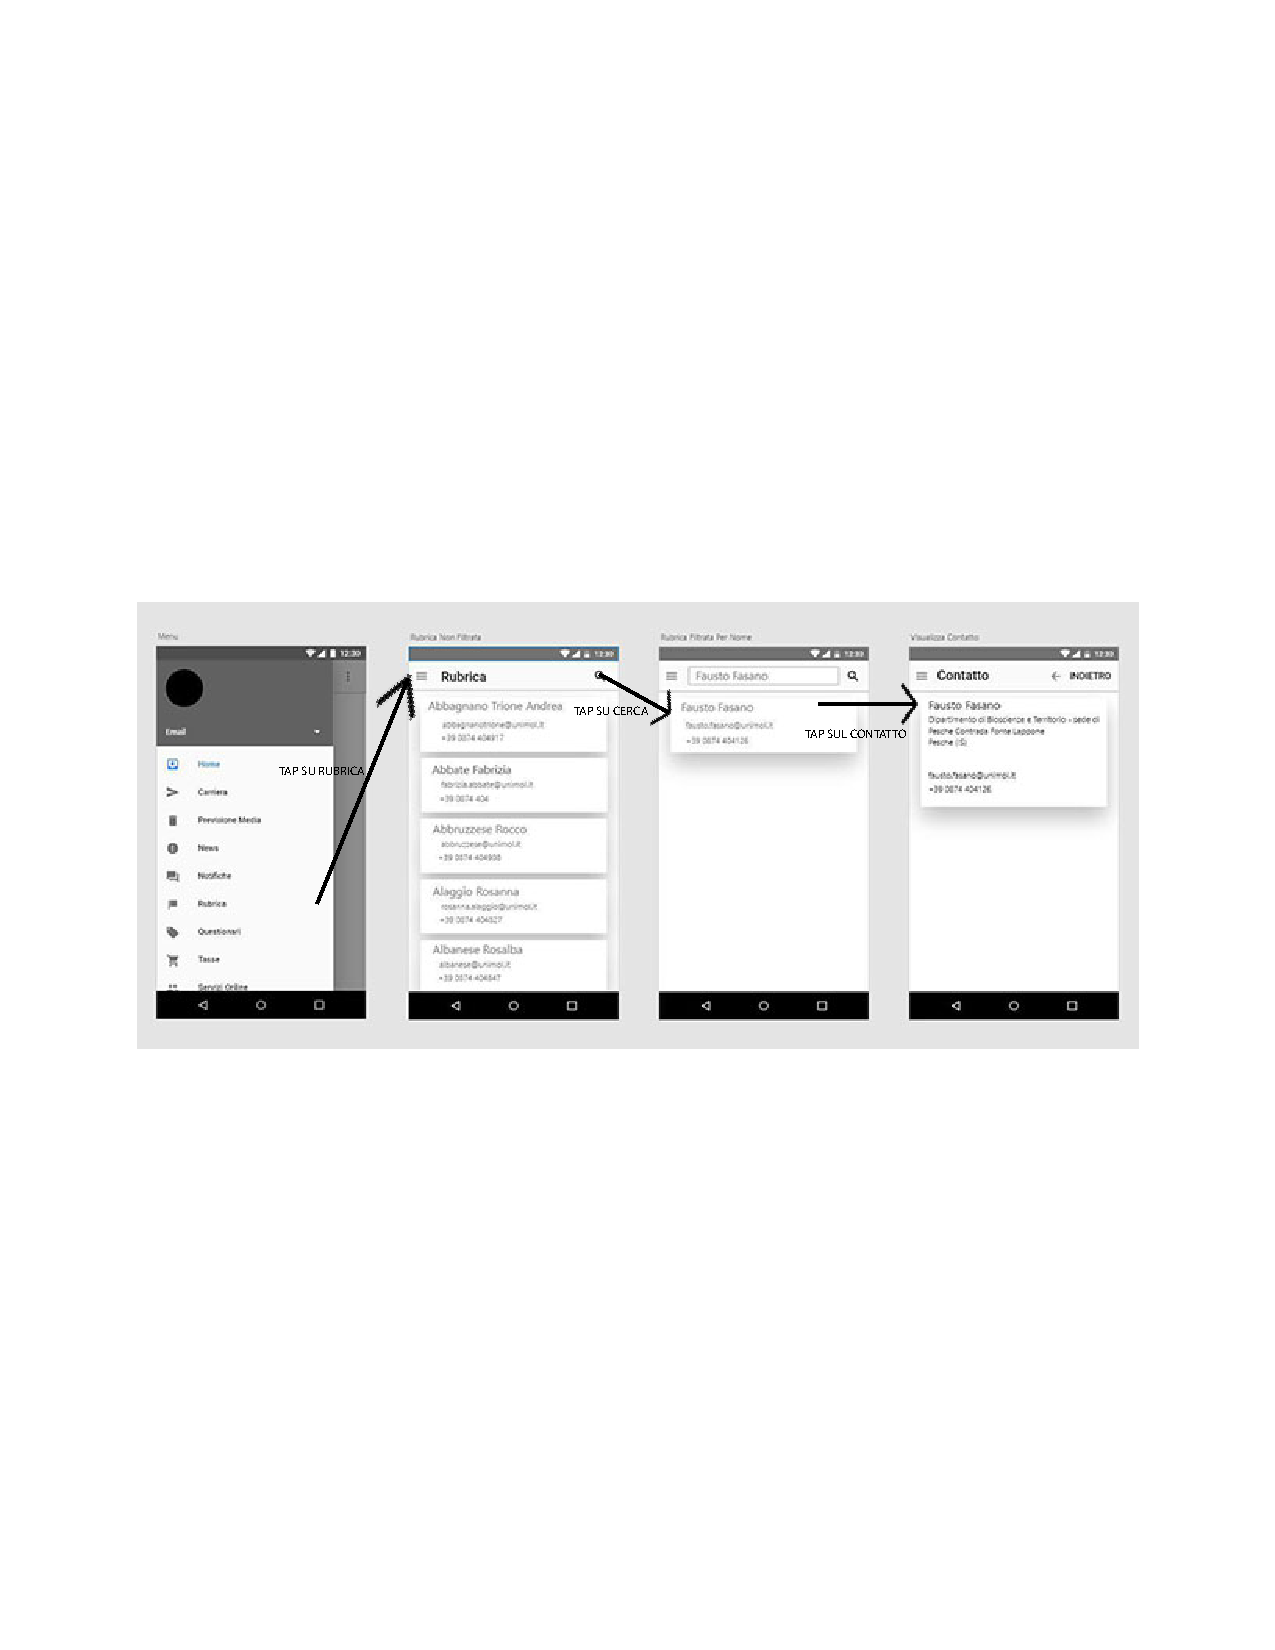
\includegraphics[height=8in,width=6in]{imgs/gruppo5/activity.pdf}
	\caption{Rubrica}
	\label{fig:prova}
\end{figure}

\clearpage